\begin{frame}
\frametitle{The surface of last scattering}
\framesubtitle{``Let there be light''}

\begin{columns}
	\begin{column}{0.25\textwidth}
		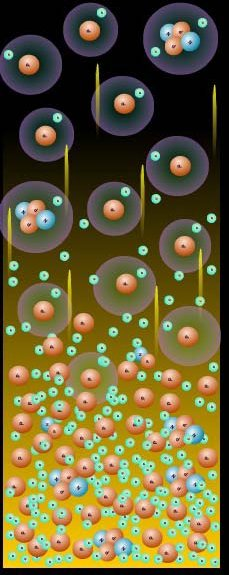
\includegraphics[width=\textwidth]{Images/last_scattering.jpg}
	\end{column}
	\begin{column}{0.75\textwidth}
	\begin{itemize}
		\pause\item At early times the universe was very dense.
		\pause\item Light could not travel through this opaque plasma.
		\pause\item At some point $\approx 3000$yrs after the big bang, the universe transitioned to being transparent to light.
		\pause\item This light was now able to travel (essentially) unimpeded, and this ``afterglow'' is what we now call the CMB.
	\end{itemize}
	\end{column}
\end{columns}

\end{frame}
